\chapter{Background}

Haskell, a purely functional language, is statically typed and lazily evaluated\footnote{\url{https://www.haskell.org/}}. As we explain above, languages with a dependent type system have no separation between types and values. In Haskell however (among other languages), programs undergo \emph{type erasure}---the executable output of the compiler has no notion of types. In other words, Haskell has a clear separation between dynamic values, and the static types those values have. Haskell separates functions over values and functions over types; it cannot be used to write functions which operate on both, like Idris can.

This is just one of the differences between Haskell's type system and a dependent type system, but it is an important one; type erasure complicates type-level programming in Haskell. This chapter summarises key aspects of Haskell's type system, including how programmers can use GHC extensions and advanced features to circumvent type erasure and perform computation at the type level in Haskell.

\section{Types in Haskell}

For a Haskell compiler, such as GHC, to accept a program, it must be well-typed (that is, every expression must have a valid type). In some cases, the type of an expression can be inferred, or it can be manually annotated by the programmer (in which case the compiler must unify the annotated type with the inferred type). If the expression has no permissible type, or if its' inferred type does not match its programmer-annotated type, then the compiler is responsible for generating a type error.

For instance, as in many other languages, one of the possible types for \inline{3} is \inline{Int}. It would be incorrect to declare an expression of a different type, and to give it a value of \inline{3}, as below:

\begin{lstlisting}
x :: Bool
x = 3  -- error: Couldn't match expected type 'Bool' with actual type 'Int'
\end{lstlisting}

However, Haskell has support for \emph{polymorphism}; firstly, parametric polymorphism, where a value's type is dependent on one or more \emph{type variables}. Consider the list type; it would be wasteful to define an entirely new list data type for each potential inhabitant. As such, the list type in Haskell is more general, in that it can hold any value of any type, provided that all elements of the list are of the same type. For instance, a list of booleans, such as \inline{[True, False]}, has type \inline{[Bool]}, which is notated as \inline{[True, False] :: [Bool]}.

In Haskell, type variables are conventionally named as lowercase single letters in alphabetical order; so the first general type in an type annotation is typically \inline{a}, followed by \inline{b}, \inline{c}, and so on. All Haskell types start with a capital letter, so any lowercase string is a valid type variable name (except for keywords). As such, the polymorphic empty list \inline{[]} has type \inline{[a]}, where the type variable \inline{a} can be unified with other types, such as \inline{Bool} in the example above.

Secondly, Haskell supports ad-hoc polymorphism, whereby functions can be specialised to operate on specific types, with separate function definitions for each type. Haskell achieves this through \emph{type classes}, a feature which is akin to interfaces in object oriented languages. We give an example below, involving the basic equality operator in Haskell (which is a member of the \inline{Eq} typeclass), with definitions for both \inline{Bool} and \inline{Int}:

\begin{lstlisting}
class Eq a where
    (==) :: a -> a -> Bool

instance Eq Bool where
    True  == True  = True
    False == False = True
    True  == False = False
    False == True  = False

instance Eq Int where
    0 == 0 = True
    0 == y = False
    x == 0 = False
    x == y = if x > 0 then (x - 1 == y - 1) else (x + 1 == y + 1)
\end{lstlisting}

Haskell functions are of the form \inline{a -> b}, for some type variables \inline{a} and \inline{b} which can unify with any other type, including function types. For instance, Boolean logical AND would have the type \inline{Bool -> Bool -> Bool}, while logical NOT would have the type \inline{Bool -> Bool}.

All Haskell functions can be curried~\cite{currying}; as an example, assume the definition of a function \inline{and}, which performs logical AND on its two inputs. The type of \inline{and} would be \inline{Bool -> Bool -> Bool}, while the type of \inline{and True} would be \inline{Bool -> Bool}, and the type of \inline{and True False} would just be \inline{Bool}. The expression \inline{and True} is well-typed, and would compile; contrasting with other languages such as C or Java, in which functions cannot be partially applied and an analogous expression (e.g. \inline{and(True)}) would fail with a type error.

Haskell allows the programmer to define their own data type with the keyword \inline{data}. These data types are \emph{algebraic}, meaning that they are types comprised of other types. For instance, to define a "Hand" type, where each finger can hold a value, the definition would be something like as follows:

\begin{lstlisting}
data Hand a = One a
            | Two a a
            | Three a a a
            | Four a a a a
            | Five a a a a a
\end{lstlisting}

However, this definition syntax has limitations; all of the return values of the type constructors above must be \inline{Hand a}. A GHC extension allows the definition of \emph{Generalised Algebraic Data Types} (GADTs)~\cite{gadts} which allows more complex type constructor definitions. The above \inline{Hand} datatype could be expressed thus:

\begin{lstlisting}
data Hand a where
    One   :: a -> Hand a
    Two   :: a -> a -> Hand a
    Three :: a -> a -> a -> Hand a
    Four  :: a -> a -> a -> a -> Hand a
    Five  :: a -> a -> a -> a -> a -> Hand a
\end{lstlisting}

Furthermore, if you wished to modify \inline{Hand} to ensure that it always stored \inline{Int} values on odd fingers, and \inline{Bool} values on even fingers, you can achieve that with GADTs like so:

\begin{lstlisting}
data Hand a where
    One   :: Int  -> Hand Int
    Two   :: Bool -> Int  -> Hand Bool
    Three :: Int  -> Bool -> Int  -> Hand Int
    Four  :: Bool -> Int  -> Bool -> Int  -> Hand Bool
    Five  :: Int  -> Bool -> Int  -> Bool -> Int  -> Hand Int
\end{lstlisting}

\section{Type-level Programming} \label{typelevelprogrammingbackground}

While GADTs are certainly useful, they are not enough to achieve type-level computation. Luckily, there are many more GHC extensions, some of which bring the language closer to have a dependent type system. In this section, we explain those used in Chesskell, to aid understanding.

\subsection{Kind Promotion} \label{promotionsection}

A key concept in type-level programming in Haskell is that of \emph{promotion}~\cite{givingpromotion}. The custom data types that programmers define (as we explain above) can be promoted to \emph{kinds}. Kinds are, conceptually, the types of types; that is, values have types, and types have kinds. A type of kind \inline{*} takes no type variables, and a type of kind \inline{* -> * -> *} takes in two type variables and returns a type. Consider an empty list, which takes a type variable; it has kind \inline{* -> *}, while the kind of a Boolean list (\inline{[Bool]}) is \inline{*}.

The kind \inline{*} is commonly aliased as \inline{Type}, since it is the kind of types which have runtime values. That distinction becomes important when promotion is involved; programmers can define their own kinds with the \inline{-XDataKinds} extension enabled. Consider a custom \inline{Book} data type, which is either \inline{Fiction} or \inline{NonFiction}. A type definition may look as follows, with either regular or GADT syntax:

\begin{lstlisting}
data Book = Fiction | NonFiction

data Book where
    Fiction :: Book
    NonFiction :: Book
\end{lstlisting}

With the \inline{-XDataKinds} extension enabled, the above code not only produces the two values \inline{Fiction} and \inline{NonFiction} with type \inline{Book}, but also two new \emph{types}: \inline{'Fiction} and \inline{'NonFiction}, of kind \inline{Book}. The key point of understanding is that there are no values of type \inline{'Fiction} or \inline{'NonFiction}---they exist solely at the type level. See \cref{promotiondiagram} for a graphical representation; note that the type \inline{Book} has kind \inline{*}, as it is a type with associated values.

\begin{figure}
    \centering
    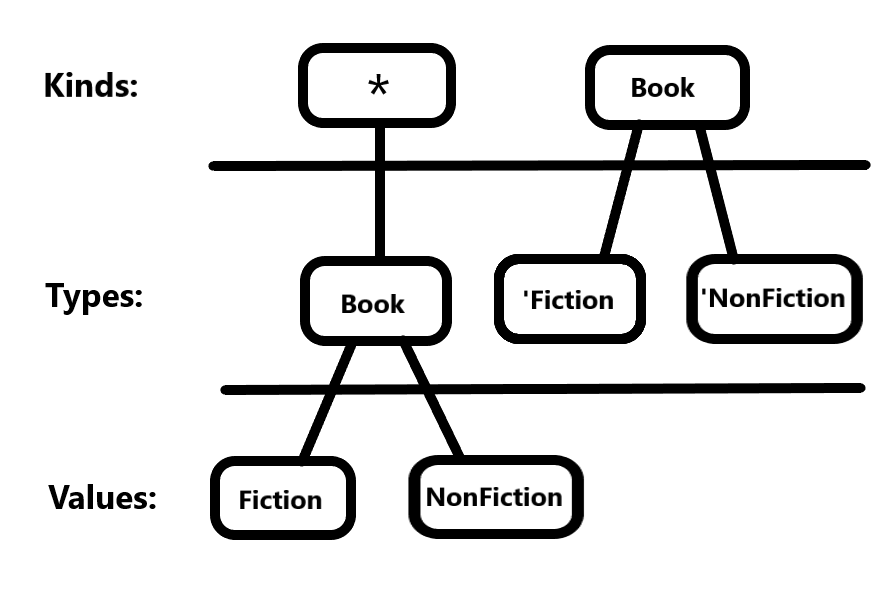
\includegraphics[width=0.8\textwidth,keepaspectratio]{Promotion.png}
    \label{promotiondiagram}
    \caption{A visual representation of the datatype promotion of the \inline{Book} type.}
\end{figure}

The syntax for "has type" and "has kind" is in both cases \inline{::}, which is unfortunate; however, in the rest of the document, where the distinction is unclear, it shall be made so. Additionally, the prefix \inline{'} for promoted types is optional, and can be left out where the compiler can unambiguously state whether an expression should be a type or a value.

\subsection{Type Families}

Another key extension introduces \emph{type families}~\cite{opentfs,closedtfs}. Type families allow the programmer to compute over types just as functions compute over values; they are the type-level analogue to functions, and come with their own syntax. Following on from the \inline{Book} example above, consider a type family \inline{IsFiction}, which states whether a given \inline{Book} is fiction or not. A value-level definition could be as follows:

\begin{lstlisting}
isFiction :: Book -> Bool
isFiction Fiction    = True
isFiction NonFiction = False
\end{lstlisting}

And the type family analogue is thus, where \inline{::} below means "has kind":

\begin{lstlisting}
type family IsFiction (x :: Book) :: Bool where
    IsFiction 'Fiction    = True
    IsFiction 'NonFiction = False
\end{lstlisting}

Both function and family use pattern-matching, and although the type family syntax is a little more verbose, it is still clear. However, the above is a \emph{closed} type family; programmers can define \emph{open} type families which can be extended beyond their initial definition. This mimics ad-hoc polymorphism, in that different implementations of the same type family can be offered with different input kinds.

There are more notable differences between (closed) type families and functions beyond syntax. The most important is that type families cannot be partially applied in the same way that functions can. Consider a function (and closed type family) \inline{IsEitherFiction}, which takes in two books and states whether either of them are fiction or not. A function definition, and a closed type family definition, are below:

\begin{lstlisting}
isEitherFiction :: Book -> Book -> Book
isEitherFiction Fiction _ = True
isEitherFiction NonFiction Fiction = True
isEitherFiction NonFiction NonFiction = False

type family IsEitherFiction (x :: Book) (y :: Book) :: Bool where
    IsEitherFiction 'Fiction _ = True
    IsEitherFiction 'NonFiction 'Fiction = True
    IsEitherFiction 'NonFiction 'NonFiction = False
\end{lstlisting}

While the function \inline{isEitherFiction} can be partially applied, the corresponding type family \inline{IsEitherFiction} cannot. One could feasibly map \inline{isEitherFiction} over a list of books, but mapping with the type family \inline{IsEitherFiction} is impossible. Imagine a type family \inline{Map}, of kind \inline{(a -> b) -> [a] -> [b]}, analogous to the value-level function \inline{map}. While the value-level expression \inline{map (isEitherFiction NonFiction) [NonFiction, Fiction]} evaluates to \inline{[False, True]}, the type-level equivalent (\inline{Map (IsEitherFiction 'NonFiction) '[ 'NonFiction, 'Fiction ]}) causes a type error. Much of functional programming relies on partial application, but these design patterns are impossible when using Haskell's Type Families.

\subsection{First-Class Families} \label{fcfbackground}

The above problem is still an open one in type-level programming, but one solution comes from Li-yao Xia, who put together a Haskell library named First Class Families\footnote{\url{https://github.com/Lysxia/first-class-families}}. First Class Families allow the programmer to map over structures, and specialise type families (a la ad-hoc polymorphism), similar to value-level functions. Sadly, First Class Families is not supported by any formal literature on the topic at the time of writing; so we briefly introduce and explain the concept below.

The key idea of this approach is the observation that, while type families cannot be partially applied, type constructors can be. Therefore, by defining type constructors along with a type-level interpreter for them, we can simulate partial type application. It relies on a type, \inline{Exp}, and an open type family, \inline{Eval}. They are defined like so:

\begin{lstlisting}
type Exp a = a -> *
type family Eval (e :: Exp a) :: a
\end{lstlisting}

Passing around the types as \inline{Exp} types allows the programmer to partially apply, and to evaluate whenever they choose with a call to \inline{Eval}. For instance, consider the \inline{IsEitherFiction} type family, but defined in "First Class Family" style instead:

\begin{lstlisting}
data IsEitherFiction :: Book -> Book -> Exp Bool
type instance Eval (IsEitherFiction Fiction Fiction) = True
type instance Eval (IsEitherFiction Fiction NonFiction) = True
type instance Eval (IsEitherFiction NonFiction Fiction) = True
type instance Eval (IsEitherFiction NonFiction NonFiction) = False
\end{lstlisting}

We can also define a type-level equivalent of \inline{map} using this technique:

\begin{lstlisting}
data Map :: (a -> Exp b) -> f a -> Exp (f b)
type instance Eval (Map f '[]) = '[]
type instance Eval (Map f (x ': xs))
    = Eval (f x) ': Eval (Map f xs)
\end{lstlisting}

When combined with the above definition of \inline{Map}, mapping (and general Functor behaviour) at the type level becomes possible with the use of \inline{Eval} -- the below expression evaluates to the type \inline{'[ 'False, 'True ]}:

\begin{lstlisting}
Eval (Map (IsEitherFiction 'NonFiction) '[ 'NonFiction, 'Fiction ])   
\end{lstlisting}

Since we use an open type family for the interpreter, there cannot be any overlapping cases as the instances are not ordered. For instance, GHC fails to compile the following definition because \inline{x} could be \inline{'Fiction} or \inline{'NonFiction} and therefore, if \inline{x} were \inline{'Fiction}, either the first or second instance shown below could apply:

\begin{lstlisting}
data IsEitherFiction :: Book -> Book -> Exp Bool
type instance Eval (IsEitherFiction Fiction _) = True
type instance Eval (IsEitherFiction x Fiction) = True
type instance Eval (IsEitherFiction x NonFiction) = False
\end{lstlisting}

When using a closed type family, or a value-level function, the definitions written are implicitly ordered. If instances overlap, the behaviour is to default to the first definition that matches. In Chesskell, we leverage this capability and combine First Class Families with closed type families, where the latter provide the actual implementation of instances of the \inline{Eval} type family. This allows us to have both partial application and the benefits of ordered definitions:

\begin{lstlisting}
data IsEitherFiction :: Book -> Book -> Exp Bool
type instance Eval (IsEitherFiction x y) = IsEitherFiction' x y

type family IsEitherFiction' (x :: Book) (y :: Book) :: Bool where
    IsEitherFiction' 'Fiction _ = True
    IsEitherFiction' x 'Fiction = True
    IsEitherFiction' x 'NonFiction = False
\end{lstlisting}

As part of the development of Chesskell, we have re-implemented many functions from Haskell's standard library using the First Class Family technique. If a First Class Family in the following sections has the same name as a function from Haskell standard library, the reader may assume that the First Class Family has similar behaviour as the value-level equivalent, unless explicitly stated otherwise.

\subsection{Type Applications}

The \inline{-XTypeApplications} Haskell syntax provides a way for the programmer to directly specify type variables~\cite{typeapplication}. Consider an empty list, with type \inline{[a]}. Using type application syntax, where we prefix a type name with \inline{@}, one can specify the type of an empty list by stating what type should inhabit type variable \inline{a}.

For example: the empty list \inline{[] @Int} has type \inline{[Int]}, and the empty list \inline{[] @Bool} has type \inline{[Bool]}. Note that the empty list value has been used in both cases; the thing that has changed is the type of that empty list.

\subsection{Proxies and Singletons}

While promotion and type families allow the programmer to compute at the type level, there must be some way to share information between the value level and the type level for this to be useful. For Chesskell, this communication only needs to be one-way; the value-level EDSL passes information up to the type system, which either compiles successfully or throws a type error. Promoted types (such as \inline{'Fiction}) have no runtime values, and so cannot be used as value-level function argument types. There are two widely used methods of circumventing this limitation in Haskell to mimic values with these promoted types; \emph{proxies} and \emph{singletons}.

\subsubsection{Proxy Types}

Proxy types provide a wrapper to allow arbitrary types to have kind \inline{*}. As we explain above, all value-level functions take in values, and all values have types with kind \inline{*}. The \inline{Proxy} type constructor takes in a single type variable, and exposes a polymorphic value \inline{Proxy}. The \inline{Proxy} type constructor, when applied to some type, has kind \inline{*}. To follow on from the previous \inline{Book} example, while \inline{'NonFiction} has kind \inline{Book}, \inline{Proxy 'NonFiction} has kind \inline{*}, and so a \inline{Proxy} value of type \inline{Proxy 'NonFiction} can be used in value level function definitions. Using the type application syntax we explain above, we can pass around type variables with arbitrary kinds using \inline{Proxy} values.

\subsubsection{Singletons}

As helpful as proxy types can be, they have one limitation; since all the value-level code sees are \inline{Proxy} values, all of the relevant information is only available at the type-level. However, singleton types~\cite{singletons} provide an alternative approach. Each singleton type has a single inhabitant value, and each individual value has a single unambiguous type. The types are mirrored in the terms, allowing similar behaviour to dependent types.

This is achieved through, for each defined type, running it through the \textit{singletons} library's Template Haskell definitions\footnote{\url{https://hackage.haskell.org/package/singletons}}. Template Haskell is a compile-time meta-programming system, similar to macros in that it allows programmers to define programs to modify and generate Haskell source code~\cite{templatehaskell}. The singletons library uses Template Haskell to define new data types, given data type definitions. Should \textit{singletons} be given the definition of the \inline{Book} datatype which we detail in \cref{promotionsection}, it will generate a new \inline{SBook} datatype, defined as below:

\begin{lstlisting}
data SBook :: Book -> * where
    SFiction    :: SBook 'Fiction
    SNonFiction :: SBook 'NonFiction
\end{lstlisting}

Due to datatype promotion, this introduces new values, types, and kinds. The runtime value \inline{SFiction} has the type \inline{SBook 'Fiction}, and the type \inline{'SFiction} has kind \inline{SBook Fiction}. These definitions are designed to enable the programmer to access type information through values, and vice versa.

The type of \inline{SNonFiction} can only be \inline{SBook 'NonFiction}, and so value-level code now has some intuition of types; and conversely, when given a type \inline{SBook a}, type families can use the type variable \inline{a} which will be either \inline{'Fiction} or \inline{'NonFiction}.

Chesskell does not make use of singletons; since the Chess rule checking is all done at the type level, there is no need to mirror the types in the values.